% !TEX root = ../../Beamer/statikz2018/statikz2018.tex

\tikz[scale=\scale]{

 \footnotesize

 \def\hi{0.1875};
 \def\radii{\hi}
 \def\extend{\hi}

 \coordinate (A) at (0,0);
 \coordinate (B) at (5,2.5);
 \coordinate (C) at (9.5,1.5);
 \coordinate (F) at (2,2.5);
 \coordinate (R) at (6.25,2.5);
 \coordinate (G) at ($ (F)!0.55!(B)+(0,1.125) $);

 \gettikzxy{(A)}{\ax}{\ay}
 \gettikzxy{(B)}{\bx}{\by}
 \gettikzxy{(C)}{\cx}{\cy}
 \gettikzxy{(F)}{\fx}{\fy}
 \gettikzxy{(R)}{\rx}{\ry}
 \gettikzxy{(G)}{\gx}{\gy}

 % \fill[white] (-3,-3) rectangle (12.5,2);

 \node[inner sep=0pt] (logo) at (\bx-.55cm,\by+1.185cm)
 {
  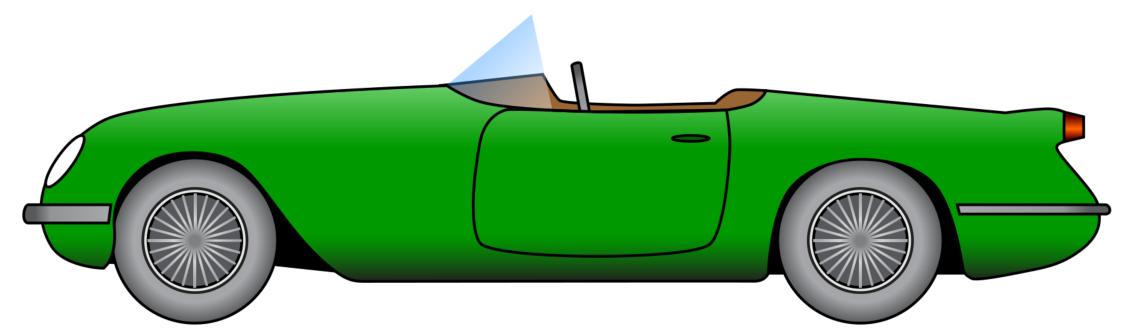
\includegraphics[scale=0.335]{../../images/greenSportsCar.png}
 };

 \shade[top color=Honeydew3, bottom color=white] (\ax-2.5 cm,\by+\hi cm) -- (\ax-0.5cm,\by+\hi cm) --  ++(-1, -1) -- ++(-1,0) -- (\ax-2.5 cm,\by+\hi cm);
 \shade[right color=Honeydew3, left color=white] (\ax-.5 cm,\by+\hi cm) -- (\ax-0.5cm,\ay-0.5 cm) --  ++(-1, -1) -- (\ax-1.5 cm,\by-1cm +\hi cm) -- (\ax-.5 cm,\by+\hi cm);
 \shade[top color=Honeydew3,bottom color=white] (\ax-0.5cm, \ay-0.5 cm) -- (\cx+\hi+0.5 cm,\ay-0.5cm) -- +(1,-1) -- (\ax-1.5 cm, \ay-1.5cm) -- cycle;
 \shade[left color=Honeydew3, right color=white] (\cx+\hi+0.5 cm,\ay-0.5cm) -- (\cx+\hi+0.5 cm,\by+\hi cm) --  ++(1, -1) -- (\cx+1.5 cm,\ay-1.5cm) -- (\cx+\hi+0.5 cm,\ay-0.5cm);
 \shade[top color=Honeydew3,bottom color=white] (\cx+0.5cm, \by+\hi cm) --  (\cx+2.5cm, \by+\hi cm)-- ++(0,-1) -- ++(-1,0)-- (\cx+0.5cm, \by+\hi cm);

 \draw[black, line width=0.1875mm] (\ax-2.5 cm, \by+\hi cm) -- (\ax-0.5 cm, \by+\hi cm)  -- (\ax-0.5 cm, \ay-0.5 cm) -- (\cx+\hi+0.5 cm,\ay-0.5cm) -- (\cx+0.5cm, \by+\hi cm) -- ++(2,0);

 \PinnedConnection[90]{C}{Honeydew3}{black}{0.5}{0.1875}
 \PinnedConnection{A}{Honeydew3}{black}{0.5}{0.1875}			%

 \filldraw[fill=Honeydew3, draw=black, line width=0.1875mm] (\bx,\by+\hi cm) -- (\cx+\hi cm, \by+\hi cm) -- (\cx+\hi cm, \cy)arc(0:-180:\hi) -- (\cx-\hi cm,\by-\hi cm) -- (\bx, \by-\hi cm) arc(-90:-270:\hi);

 \filldraw[fill=Honeydew3, draw=black, line width=0.1875mm] (\ax-\hi cm,\ay) -- (\ax-\hi cm, \by+\hi cm) -- (\bx, \by+\hi cm)arc(90:-90:\hi) -- (\ax+\hi cm,\by-\hi cm) -- (\ax+\hi cm, \ay) arc(0:-180:\hi);

 \shadedraw[ball color=Honeydew3] (A) circle (3pt);
 \shadedraw[ball color=Honeydew3] (B) circle (3pt);
 \shadedraw[ball color=Honeydew3] (C) circle (3pt);
 \shadedraw[ball color=black] (G) circle (3pt);

 \draw (\ax,\ay-1.125cm) -- (\ax,\ay-2.5cm);
 \draw (\bx,\by-0.75cm) -- (\bx,\ay-2.5cm);
 \draw (\cx,\cy-0.75cm) -- (\cx,\ay-2.5cm);
 \draw (\rx,\ry-0.75cm) -- (\rx,\ay-2.5cm);
 \draw (\fx,\fy-0.75cm) -- (\fx,\ay-2.5cm);
 \draw (\gx,\gy-0.375cm) -- (\gx,\ay-2.5cm);
 %
 \draw (\cx-1.5cm,\cy) -- (\cx-0.375cm, \cy);
 \draw (\ax+0.375cm,\ay) -- (\cx-0.375cm,\ay);
 \draw (\cx-1.5cm,\by) -- (\cx-0.375cm, \by);

 \draw[latex-latex] (\ax,\ay-2.25cm) -- node[fill=white, inner sep=0.3mm]{$1.000\>\text{m}$}(\fx,\ay-2.25cm);
 % \draw[Stealth-Stealth] (\fx,\ay-2.25cm) -- node[fill=white]{$2.30\>\text{m}$}(\bx,\ay-2.25cm);
 \draw[latex-latex] (\fx,\ay-2.25cm) -- node[rotate=45, fill=white, inner sep=0.3mm]{$0.825\>\text{m}$}(\gx,\ay-2.25cm);
 \draw[latex-latex] (\gx,\ay-2.25cm) -- node[rotate=45, fill=white, inner sep=0.3mm]{$0.675\>\text{m}$}(\bx,\ay-2.25cm);
 \draw[latex-latex] (\bx,\ay-2.25cm) -- node[rotate=45, fill=white, inner sep=0.3mm]{$0.625\>\text{m}$}(\rx,\ay-2.25cm);
 \draw[latex-latex] (\rx,\ay-2.25cm) -- node[fill=white, inner sep=0.3mm]{$1.125\>\text{m}$}(\cx,\ay-2.25cm);

 \draw[latex-latex] (\bx*0.2+\cx*0.8,\by) -- node[fill=white, inner sep=0.25mm]{$0.500\>$m}(\bx*0.2+\cx*0.8,\cy);
 \draw[latex-latex] (\bx*0.2+\cx*0.8,\cy) -- node[fill=white]{$0.750\>$m}(\bx*0.2+\cx*0.8,\ay);

 \node[yshift=-0.55cm] at (A) {\large $A$};
 \node[yshift=-0.3125cm] at (B) {\large $B$};
 \node[yshift=-0.3125cm] at (C) {\large $C$};
 \node[above left] at (G) {\large $G$};
 \node[yshift=-0.3125cm] at (F) {\large $F$};
 \node[yshift=-0.3125cm] at (R) {\large $R$};
}
